\documentclass[../../main.tex]{subfiles}

\begin{document}

% \newpage
\subsubsection{Komunikácia v IoT}
Komunikácia v IoT môže používať viacero rozličných protokolov ako RFID, AD-HOC, Ethernet, Wi-Fi, 3G, 4G, Bluetooth, ZigBee, USB, WSN, and IPv6. Pre krátku veľkosť rozsahu pripojenia sa používa napríklad Bluetooth, pre strednú WiFi, pre veľké mobilné siete.
Pre riadenie napríklad FPGA alebo procesor. Ako akčné členy sa využívajú napríklad motory alebo alarmy. Architektúra sa skladá z troch vrstiev fyzická, komunikačná a aplikačná. \cite{springerprofessional.de_The_Era_of_IoT} 

\begin{wrapfigure}{r}{0.5\textwidth}
    \centering
  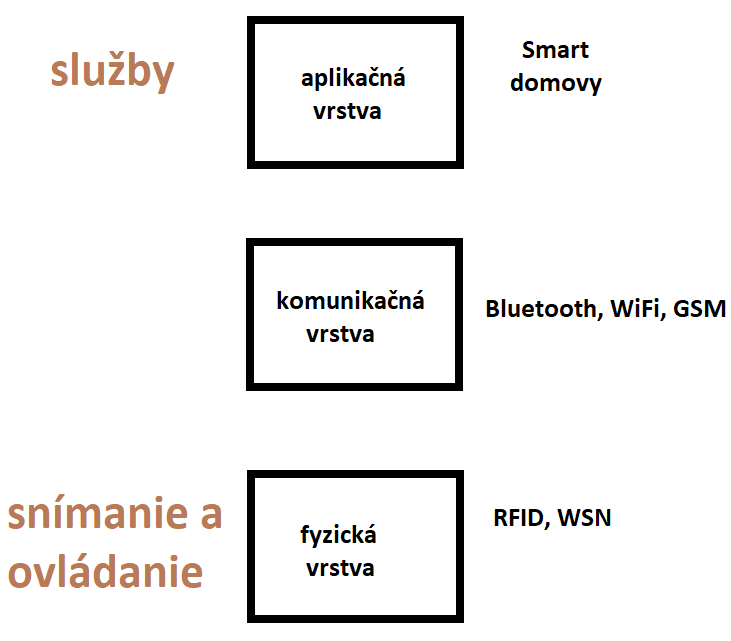
\includegraphics[width=0.47\textwidth]{images/IoT_vrstvy.png}
  \caption{IoT architektúra\cite{springerprofessional.de_The_Era_of_IoT}}
\end{wrapfigure} 
Nie každé zariadenie musí byť pripojené k internetu. Uzly IoT sú pospájané medzi sebou. Za komunikáciu s uzlami je zodpovedný Gateway v oboch smeroch, ktorý preloží dáta do JSON alebo XML a pošle dáta ďalej do siete world wide web. Opačne preloží Gateway príkazy do podporovaného formátu pre protokoly IoT  a komunikačnú technológiu.\cite{springerprofessional.de_The_Era_of_IoT}Zariadenia môžu byť adresovateľné pomocou URN(Uniform Resource Name )\cite{GUBBI20131645}
%DOPLNIT
\subsubsection{Komunikačné technológie používané v IoT}
\paragraph{Radio Frequency Identification (RFID)} umožňuje každému zariadeniu mať unikátne identifikovanie pomocou vstavaného čipu. Čipy môžu byť pasívne alebo aktívne. Pasívne nemajú batériu, dokážu len odpovedať na dopyt RFID. čítača. \cite{GUBBI20131645} RFID čipy spolu s RFID tagmi emitujú aj údaje o lokalizácií alebo inej špecifickej vlastnosti objektu.
\paragraph{Wireless Sensor Networks (WSN)} používa malé lacné, energeticky nenáročné  zariadenia používané pre vzdialené snímacie aplikácie. \cite{springerprofessional.de_The_Era_of_IoT}
WSN monitorovacia sieť zahŕňa:. \cite{GUBBI20131645} 
\begin{multicols}{2}
    \begin{itemize}
        \item WSN hardware - senzorové rozhrania, procesné jednotky a zdroje napájania \item  WSN komunikačný zásobník - vhodná topológia pre ad-hoc spojenia\item WSN Middleware - mechanizmus ako kombináciu service orientovanú architektúru a senzorovú sieť.
        %doplnit
        \item zabezpečenie zhromaždených dát \\ - schopnosť systému pracovať pri zlyhaniach
        
    \end{itemize}
\end{multicols}
\paragraph{I²C sériová zbernica}  - je multi-master, multi-slave zbernica vynájdená spoločnosťou Philips Semiconductor v roku 1982, často používaná pre pripojenie viacerých zariadení. Primárne používaná na ovládanie procesorov a mikrokontrolérov. Zbernica sa skladá z 2 liniek: SDA(serial data) a SCL(serial clock). Každá linka je pripojená k pullup rezistoru. Ovládače sú \say{open drain}, to znamená, že môžu stiahnuť signál na linke na nízku hodnotu, ale nie nastaviť na vysokú hodnotu. Takto je zabezpečená proti potencionálnemu poškodeniu\cite{sparkfun}. Zariadenie dokáže svojho zapnutím tranzistora stiahnuť hodnotu na linke na nízku hodnotu. Keď žiadne zariadenie nechce vysielať (nezníži hodnotu na linke na nízku hodnotu), signál na linke sa zmení na vysokú hodnotu vďaka pullup rezistoru. Štandard povoľuje niekoľko módov v rôznych pomeroch.\cite{WOLF201923}
\begin{multicols}{4}
    \begin{itemize}
        \item standard mode:\\ 100 kbit/s
        \item fast mode:\\ 400 kbit/s
        \item fast mode plus:\\  1 Mbit/s
        \item high speed mode:\\ 3.4 Mbit/s
    \end{itemize}
\end{multicols}
Štandard umožňuje maximálnu frekvenciu hodín 100 kHz.
\subparagraph{Prenos bitov v I²C} začína, keď master prepne z vysokej hodnoty napätia na nízku hodnotu pred prepnutím vysokej hodnotu na nízku na linke SCL pre každé pripojené zariadenie.
Ďalej master odošle 7 alebo 10 bitovú adresu zariadenia s ktorým chce komunikovať spolu s read/write bitom. Každé slave zariadenie si skontroluje poslanú adresu s vlastnou, ak sa zhoduje, slave odpovedá ACK bitom znížením hodnoty na nízku na linke SDA. Zhodnú adresu môže mať aj viac zariadení naraz. V tom prípade získava komunikáciu zariadenie, ktoré rýchlejšie odpovedá\cite{i2c_protocol}. Ostatné zariadenia nechávajú  SDA linku na vysokej hodnote napätia. Začne sa prenos data rámca. Prvý je vyslaný MSB (most-significant bit), posledný LSB (least-significant bit). Po každom ukončenom prenesenom rámci prijímateľ odošle ACK bit odosielateľovi. Pre ukončenie prenosu master odošle zastavovaciu podmienku zvýšením hodnoty napätia na linke SCL pred zmenou na vysokú hodnotu napätia na linke SDA.
\pageref{fig:i2c_message}
V zbernici môže byť aj viac master zariadení. V prípade konfliktu vysiela dáta na linku master s vyššou prioritou\cite{WOLF201923}. Zbernica je pomalšia a vyžaduje zložitejší hardvér ako SPI.\cite{i2c_protocol}
Na obrázku Obr. \ref{fig:i2c_message} zo strany \pageref{fig:i2c_message} je zobrazené zloženie správy I²C protokolu.

\begin{figure}[htbp!]
    \centering
  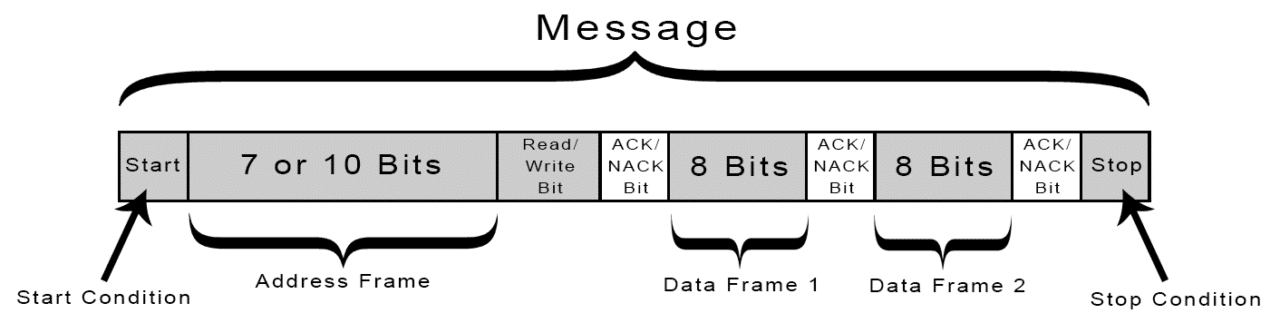
\includegraphics[scale=0.4]{images/I2C-Message-Frame-and-Bit-2.png}
  \caption{I²C správa \cite{i2c_protocol}}
    \label{fig:i2c_message}
\end{figure} 
%mozno dopisat natiahnutie hodin, opakovane posielanie bitov, multimaster
\paragraph{USB - Universal Serial Bus} je používaná väčšinou zariadení informačnej techniky. Na tabuľke č. \ref{table:USB_ALZA} na strane \pageref{table:USB_ALZA} sú zobrazené štandardy s ich prenosovými rýchlosťami. USB zariadenia pripojené na zbernicu poskytujú aplikáciám bežiacim na USB host zariadeniu funkcie. Aplikácie používajú USB API. Fyzicky je USB zbernica zobrazená ako strom, kde je koreň stromu host(root hub). USB 2.0 používa 4 káble na pripojenie uzla do siete: zdrojový, uzemňovací a dva dátové káble. Hodinový signál je zakódovaný spolu s dátami. Lepšie štandardy môžu obsahovať aj viac dátových káblov. Host controller inicializuje všetky prenosy. Prenos obsahuje buď tok dát alebo správ(požiadavky).Ďalej sa prenosy delia na kontrolné, izochrónne, prerušenia, dávkové prenosy. Komunikácia na zbernici je rozdelená do paketov. Bajty sú posielané vo formáte little-endian, LSB  bit je posielaný prvý. Paket sa delí na časti: SYNC pole, identifikátor PID, adresa funkcie, koncový bod, číslo rámca, pole dát (0-1024 bajtov)
a CRC(cyclic redundancy check). Zariadenie môže byť v jednom z nasledujúcich stavov: ATTACHED, POWERED, DEFAULT(reset), ADDRESS(pridelené host kontrolérom), CONFIGURED, a môže byť suspendované, keď už host nepoužíva jeho funkcie. Po pripojení zariadenia host kontrolér zaregistruje udalosť na svojom kanáli(pipe). Host sa dopytuje cez hub po identifikácií portu a  určení zmeny, zariadenie je v stav ATTACHED, host čaká najmenej 100ms, kým sa zapne zariadenie (stav POWERED), host vyžaduje zresetovanie portu, stav zariadenia je DEFAULT. Host skontroluje maximálnu kapacitu dát pre zariadenie pomocou kontrolného kanálu, host pridelí unikátnu adresu zariadeniu, zariadenie je v stave ADDRESS. Host skontroluje konfiguráciu pre zariadenie, po vykonanej potrebnej konfigurácií je v stave configured. Niektoré operácie sú limitované časom. Host používa USB systémový softvér, ktorý sa skladá z ďalších komponentov. \cite{WOLF201923}

\begin{table}[h!]
\begin{tabular}{|c|c|c|}
\hline
\textbf{Štandard} &
\textbf{Prenosová rýchlosť}&
\textbf{Poznámka}\\
\hline
USB 1.0
&
Low Speed (1,5 Mbit/s), Full Speed (12 Mbit/s)
& \\
\hline
USB 2.0
&
High Speed (480 Mbit/s)
& \\
\hline
USB 3.0
&
SuperSpeed USB (5 Gbit/s)
&
Označenie USB 3.2 Gen 1
\\
\hline
USB 3.1
&
SuperSpeed USB 10 Gbps (10 Gbit/s)
&
Označenie USB 3.2 Gen 2
\\
\hline
USB 3.2
&
SuperSpeed USB 20 Gbps (20 Gbit/s)
&
Označenie USB 3.2x2 
\\
\hline

\end{tabular}
\caption{Štanadrdy USB a ich prenosové rýchlosti\cite{USB_ALZA}}
\label{table:USB_ALZA}
\end{table}
%doplnit kodovanie pri rôznych štandardoch, kable, 

\paragraph{Wireless LANs} - bezdrôtové siete LAN, takáto komunikácia sa začala na Havajských Ostrovoch, používajú hlavne štandard IEEE 802.11. Využívajú buď infraštruktúru AP (Access Point), alebo menej používaný ad-hoc network. Pri AP klienti posielajú a prijímajú pakety cez prístupový bod AP, pri ad-hoc komunikuje skupina počítačov medzi sebou zaťažuje sieť, takže táto metóda nieje veľmi populárna. Všetky techniky 802.11 používajú na komunikáciu krátke vlny buď pásma 2,4GHz alebo 5GHz.
802.11 sa líšia od ostatných ethernetových protokolov. Komunikácia cez vysielače môže mať len polovičný duplex, pretože vysielače nedokážu naraz vysielať aj prijímať signál kvôli vznikajúcemu šumu a vysielaný signál môže byť oveľa silnejší než prijatý. Protokoly 802.11 sa pre vyhnutie kolíziám riadia protokolom CSMA/CA
(CSMA with Collision Avoidance), ktorý zabezpečuje ktorá stanica môže kedy vysielať a kedy musí počkať. Stanice musia byť autentifikované predtým, ako posielajú dáta cez AP ale sieť môže byť aj otvorená. Odporúčaná schéma je WPA2 (WiFi Protected Access 2). Staršia schéma WEP (Wired Equivalent
Privacy), ktorá je zlomitelná a softvér na jej zlomenie je dostupný na internete. Šifrovanie pre WPA2 používa algoritmy založené na AES (Advanced Encryption Standard) - štandard schválený americkou vládou v roku 2002.\cite{tanenbaum}
% \begin{flushleft}

\paragraph{WiFi(Wireless Fidelity - ide o marketingovú náhradu pre štandard „IEEE 802.11“\cite{wifi_fontech})} je názov štandardov pre bezdrôtové dátové spojenie. WiFi sa zaoberá časť štandardov IEEE 802.11,%mozno treba doplnit citaciu 
ktorému sa WiFi Aliancia, ktorá je aj Držiteľom ochrannej značky WiFi \cite{tanenbaum,wifi_fontech}. Štandardy definujú vrstvy MAC (Medium access control) a PHY (fyzická vrstva)  pre bezdrôtové LAN. Každá verzia štandardu je kompatibilná s 802.3 Ethernet\cite{wlan_wifi_diff}. Rýchlosť sa pohybuje medzi 6-9.6 Gbit/s.\cite{wifi_fontech}. Na nasledujúcej tabuľke číslo \ref{tab:wifi_stan} zo strany \pageref{tab:wifi_stan} sú zobrazené jednotlivé štandardy a ich rýchlosti. Pre sprehľadnenie WiFi Aliancia sa rozhodla používať pre posledné štandardy IEEE 802.11n, IEEE 802.11ac a IEEE 802.11ax názvy WIFI 4,5 A 6. Posledný štandard Wi-Fi 6E môže pracovať aj vo frekvencii 6GHz, ktoré zatiaľ nie je dostupné, ale aliancia sa ho snaží získať.





\begin{table}[h]
    \centering
    \begin{tabular}{|c|c|c|c|}
        \hline
        \textbf{Generácia} &	\textbf{Rýchlosť} & \textbf{Prijatie}	& \textbf{Frekvenčné pásmo}
        \\
        \hline
        Wi-Fi 6E & 	do 9,6 Gbit/s &	2019 &	6 GHz \\
        \hline
        Wi-Fi 6	& do 9,6 Gbit/s &	2019 &	2,4 GHz a 5 GHz \\
        \hline
        Wi-Fi 5	& do 6,9 Gbit/s &	2014 &	5 GHz \\
        \hline
        Wi-Fi 4	& do 600 Mbit/s &	2009 &	2,4 GHz a 5 GHz \\
        \hline
        802.11g	& do 54 Mbit/s &	2003 &	2,4 GHz \\
        \hline
        802.11a	& do 54 Mbit/s &	1999 &	5 GHz \\
        \hline
        802.11b	& do 11 Mbit/s &	1999 &	2,4 GHz \\
        \hline
    \end{tabular}
    \caption{Wifi štandardy a ich rýchlosti\cite{wifi_fontech}}
    \label{tab:wifi_stan}
\end{table}


\paragraph{Bluetooth},
v roku 1994 sa o bezdrôtový prenos začala zaujímať spoločnosť L. M. Ericsson. Spolu so spoločnosťami IBM, Intel, Nokia, Toshiba vytvorili konzorcium SIG (Special Interest
Group) a v roku 1998 vytvorili štandard pre bezdrôtovú komunikáciu medzi mobilnými a počítačovými zariadeniami a príslušenstvom s využitím krátkych nízko-energetických vĺn. Projekt sa nazval Bluetooth. Bluetooth využíva komunikáciu párovaním. Systém bluetoothu používa základné jednotky piconety, kde sa nachádza jeden master-uzol a niekoľko slave-uzlov vo vzdialenosti do 10 m. Niekoľko prepojených takýchto piconetov cez \say{bridge} uzol vytvára sieť zvanú scatternet (Obr. \ref{fig:scatternet}, strana \pageref{fig:scatternet}). Počet aktívnych uzlov a pozastavených môže byt určitý počet v sieti piconet. Pozastavené \say{parked} uzly určuje master aby šetril ich batérie. Takéto zariadenia môžu jedine odpovedať na \say{beacon signal}(signál, ktorý indikuje blízkosť alebo pripravenosť zariadenia, takéto signály robia bezdrôtovú sieť viac inteligentnú a čitateľnú\cite{beacon_signal}) od mastera. Master určuje, ktoré zariadenie bude s ním komunikovať a sieť sa riadi podľa jeho hodinového signálu. Podľa funkcií aplikácií sú vytvorené rozličné profily, napríklad profil pre headset, hands-free alebo profily pre video, kamery, zvuk...
 \begin{wrapfigure}{L}[-8MM]{0.5\textwidth}
    \centering
  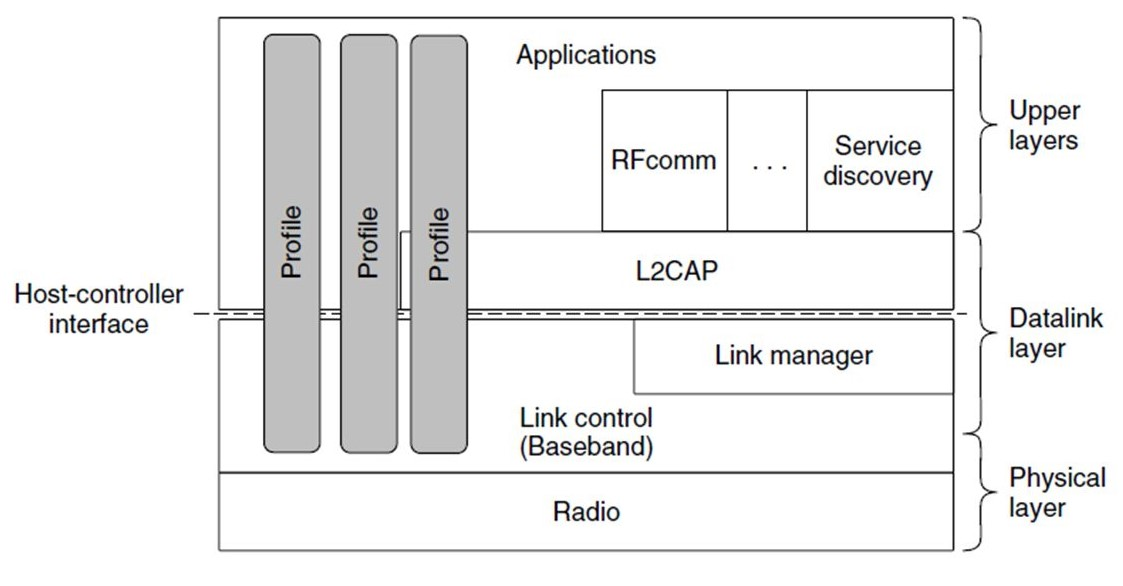
\includegraphics[width=0.48\textwidth]{images/bluetooth_stack.jpg}
  \caption{Bluetooth - protokoly\cite{tanenbaum}}
    \label{fig:bluetooth_stack}
\end{wrapfigure} 
\subparagraph{Bluetooth štandard} môžme rozdeliť do 3 vrstiev (Upper, Datalink, Physical). Protokoly sú zobrazené na Obr. \ref{fig:bluetooth_stack} na strane \pageref{fig:bluetooth_stack}. Protokoly fyzickej vrstvy, ktoré sa zaoberajú vysielaním a moduláciou. Prokokoly Datalink vrstvy: link control protokol, ktorý sa zaoberá ovládaním časových \say{slotov} a rámcami a Link manager - protokol sa zaoberá zachytávaním vytvorených kanálov medzi zariadeniami, spárovanim, šifrovaním, manažment energie a Quality of Service. Tieto protokoly zvyčajne obsahuje zariadenie, ktoré s čipom je hostiteľ danému zariadeniu. Toto zariadenie obsahuje ďalšie protokoly:
L2CAP (Logical Link Control Adaptation
Protocol - tiež Datalink vrstva), ktorý sa zaoberá vytváraním rámcov. Nakoniec najvrchnejšia vrstva (Upper), ktorá obsahuje aplikácie a RFComm protokol sa zaoberá vyhľadávaním portu na PC pre pripojenie zariadenia. V tejto a v strednej vrstve (datalink) sa nachádzajú aj profily, ktorú môžu používať rôzne protokoly z týchto dvoch vrstiev. 


 \begin{wrapfigure}{r}[-8MM]{0.4\textwidth}
 \centering
  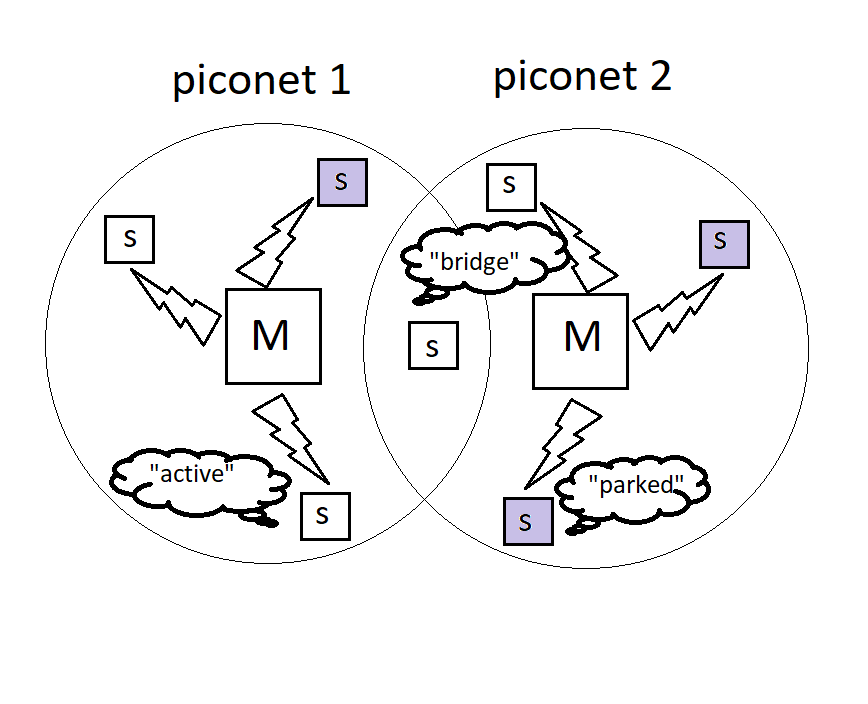
\includegraphics[width=0.38\textwidth]{images/scatternet.png}
  \caption{scatternet s 2 piconetmi a 1 spoločným uzlom\cite{tanenbaum}}
    \label{fig:scatternet}
 \end{wrapfigure}

\subparagraph{Bluetooth radiová vrstva} prenáša bity medzi master uzlom a slave uzlom alebo naopak. Pracuje s  2,4MHz ISM (The Industrial, Scientific, and Medical) frekvenciou ako 802.11 do vzdialenosti 10m. Pásmo je rozdelené na 79 pásiem po 1MHz. Aby mohol systém fungovať, frekvencia sa môže meniť v spektre niekoľko krát za sekundu. Preskoky vo frekvencií určuje master celému piconetu. Bluetooth sa snaží vyhýbať už používaným pásmam, ktoré používajú iné systémy. Len pre zaujímavosť, techniky zmeny frekvencie boli využívané armádou a spolu vynašla ich rakúska herečka Hedy Lamarr, ktorá si zahrala v českom filme Extase (1933). Keď zistila, že jej manžel predáva zbrane Hitlerovy, utiekla do USA, kde vo svojom voľnom čase pomáhala spojencom\cite{tanenbaum}.




\subparagraph{LoRaWAN®} špecifikácia je nízko príkonový sieťový protokol, s pokrytím pre veľké územia. Je navrhnutý pre pripojenie zariadení s batériami k iným sieťam. Spĺňa podmienky IoT ako obojsmerná komunikácia, bezpečnosť koncových bodov a lokalizácia. Architektúra má topológiu hviezdy. Správy sú prenášané medzi centrálnym serverom a koncovými zariadeniami pomocou gateways. Medzi serverom a gateway je použitý protokol IP (Obr \ref{fig:lorawan} strana \pageref{fig:lorawan}). Jedno zariadenie môže dosahovať viac gateways. Koncové zariadenia sa delia na 3 triedy.\\
    \textbf{Trieda A, nízky príkon, obojsmerná komunikácia medzi koncovými zariadeniami:} Musia ju spĺňať všetky zariadenia. Komunikácia sa riadi podľa protokol ALOHA.\\
    \textbf{Trieda B, Obojsmerná komunikácia s určeným oneskorením:} komunikácia je zlepšená plánovaním a synchronizovaním. Je možné programovať oneskorenie do 128 sekúnd.\\
    \textbf{Trieda C, Obojsmerná komunikácia s nízkym oneskorením:} komunikácia je half duplex. Oneskorenie je zredukované. Je možná prechádzať medzi triedami A a C.
    %https://www.quark.sk/prvy-stratosfericky-test-lorawan-siete-internetu-veci-svete-sa-uskutocni-slovensku/ ked tak doplnit a pasma
 Prenosová rýchlosť je 0.3 kbps až 50 kbps. Pre bezpečnosť je používaný algoritmus AES LoRaWAN®    špecifikácia je vyvíjaná a udržiavaná  LoRa Alianciou.\cite{lorawan}
 LoraWan dokáže komunikovať v častiach s hustejšou zástavbou vo vzdialenosť 2 km, mimo aj 20 km.\cite{WOLF201923}
 \begin{figure}[h!]
  \includesvg[scale=0.8]{images/lorawan.svg}
  \caption{LoraWan architektúra\cite{lorawan}}
    \label{fig:lorawan}
\end{figure} 

\newpage
 \begin{wrapfigure}[5]{r}{0.36\textwidth}
 \centering
  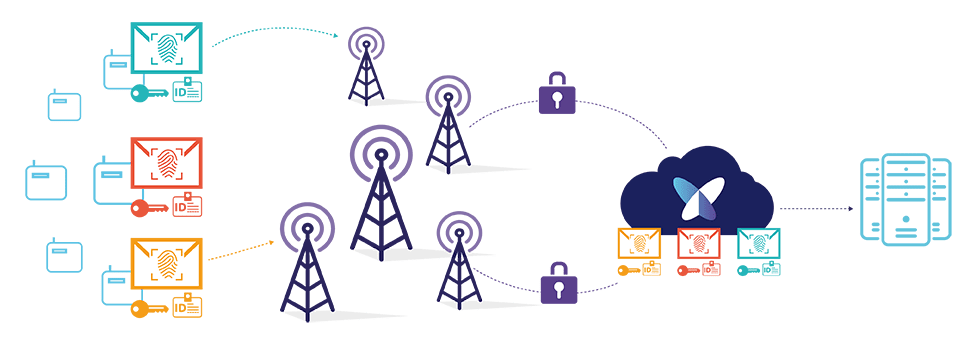
\includegraphics[width=0.35\textwidth]{images/sigfox.png}
  \caption{schéma Sigfox\cite{sigfox}}
    \label{fig:sigofx}
\end{wrapfigure}
\paragraph{Sigfox} bol vytvorený v roku 2010 dvomi francúzskymi zakladateľmi (Ludovic Le Moan a Christophe Fourtet) ako globálna sieť vhodná pre IoT, Založená na nízkom príkone, dlhom dosahu a end-to-end konektivite malých dát. Sigfox je tiež dizajnovaný pre IoT. Sigfox je prítomný vo viac ako 70 

\noindent
\begin{wrapfigure}{l}{0.45\textwidth}
 \centering
  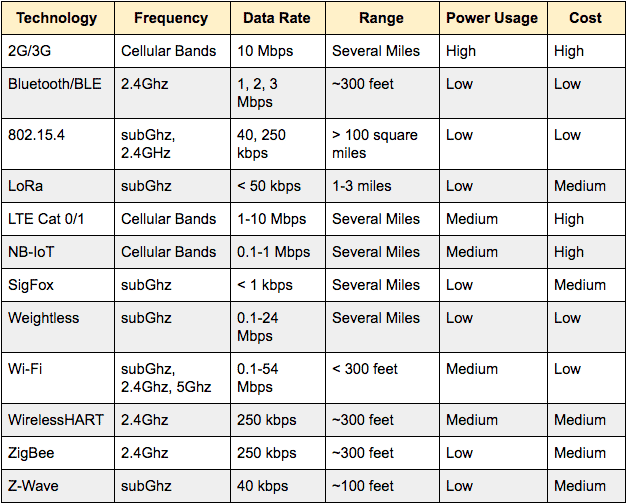
\includegraphics[width=0.44\textwidth]{images/protocols_comparasion1.png}
  \caption{Porovnanie protokolov\cite{protocols_comparasion}}
    \label{fig:sigfox1}
\end{wrapfigure}
krajinách a spolu s veľkými výrobcami a Startup-mi môže vyvinúť jeden z najväčších ekosystémov na svete. Komunikácia prebieha zaslaním správy na najbližšiu základňovú stanicu v dosahu. Správy posielané do siete majú do 12 bajtov a dosiahnutie základňovej stanice trvá priemerne 2 sekundy. Správy posielané zo siete môžu mať 8 bajtov. Cena služby bude závisieť od počtu správ a zariadení, malo by ísť však o jednotky eur za rok. Systém používa frekvenciu 868 MHz, pri ktorej vlny neprechádzajú dobre zeminou, takže pri priestoroch hlbších, ako je suterén je treba použiť lokálny vykrývač.
 
\begin{wrapfigure}{r}{0.41\textwidth}
 \centering
  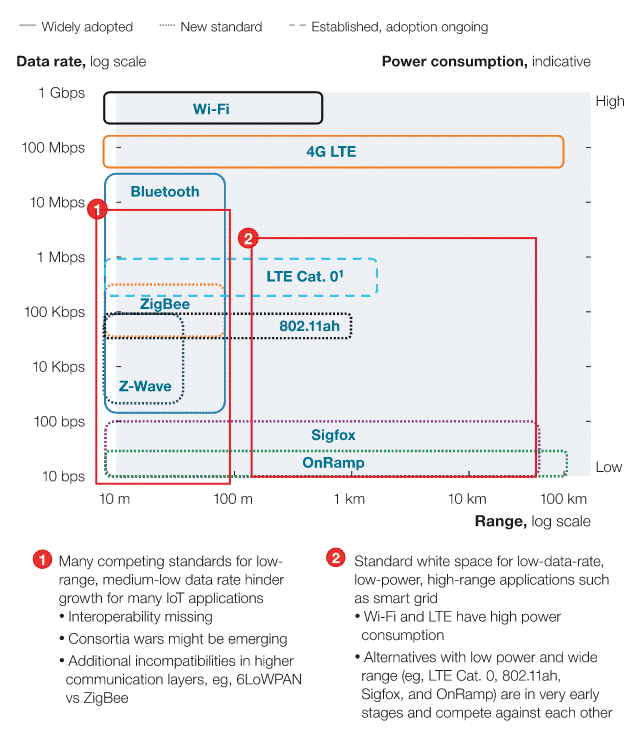
\includegraphics[width=0.4\textwidth]{images/protocols_comparasion2.png}
  \caption{Porovnanie protokolov \cite{protocols_comparasion}}
    \label{fig:sigfox2}
\end{wrapfigure}
\noindent Sigfox je stále v štandarizačnom procese.Pre moduláciu mu stačí pásmo 200 KHz. Zariadenie vysiela správy 3 krát v 3 rôznych frekvenciách. Základňová stanica monitoruje signály ultra tenkého pásma pre demoduláciu. Správu môže zachytiť viac základňových staníc. Týmito spôsobmi sa zabezpečí odolnosť systému. Zariadenie si vyberá, ktorú frekvenciu bude počúvať, čím sa zabezpečí ochrana pred útočníkmi, ktorí by mohli posielať zariadeniu správy\cite{sigfox}. Za spoločnosťou Sigfox stoja investori ako Intel, Telefonica, Samsung, Engie, Eutelsat, NTT DoCoMo, SK Telecom. Zoznam ďalších investorov je vypísaný na \url{https://www.sigfox.com/en/sigfox-board-and-investors}. Služba pokrýva aj skoro celú Slovenskú republiku\cite{sigfox_sk}.
%da sa este dopisat dalsie zigbee,nfc, cellular
Nakoniec pridávam porovnanie niekoľkých používaných protokolov používaných v IoT na Obr. \ref{fig:sigfox1} a  \ref{fig:sigfox2}.


%dorobit tabulku...zmenit ze obrazok
% \begin{table}[]
%     \centering
%     \begin{tabular}{|c|c|c|c|c|c|c|}
%         Protocol & 	Nominal Range Limit & Typical Data Rate	& Spectrum	& Power usage	Standard	Alliance	Year first launched
%         ZigBee	Local (<100m)	250 kbps	2.4 GHz	Low (<100mW)	ZigBee spec. 05-3474-21, IEEE 802.15.4-2011	ZigBee Alliance	2003
%         Z-Wave	Local (<100m)	40–100 kbps	900 MHz unlicensed	Low (<100mW)	ITU-T G.9959	Z-Wave Alliance	2003
%         Bluetooth EDR	Local (<100m)	2 Mbps	2.4 GHz	Medium (<1W)	IEEE 802.15.1	Bluetooth Special Interest Group	1999
%         Bluetooth LE	Local (<100m)	1 Mbps	2.4 GHz	Low (<100mW)	IEEE 802.15.1	Bluetooth Special Interest Group	2011
%         LoRaWAN	Metro (>10km)	<50 kbps	900 MHz unlicensed	Low (<100mW)	Proprietary	LoRa Alliance	2015
%         Sigfox	Metro (>10km)	<100 bps	900 MHz unlicensed	Low (<100mW)	Proprietary	Sigfox company	2009
%         NB-IoT	Metro (>10km)	<250 kbps	900 MHz	Low (<100mW)	3GPP Release 13	3GPP	2016
%         6LoWPAN	Local (<100m)	250 kbps	2.4 GHz	Low (<100mW)	IETF/RFC 4944, IEEE 802.15.4	6LoWPAN IETF WG	2007
%         LTE	Metro (>30km)	>100 Mbit/s	Licensed cellular	Band dependant	3GPP Release 8 and 9	GSMA - Cellular Carriers	2010
%         5G	Metro (>30km)	<10 Gbps	Licensed cellular	Band dependant	3GPP 5G	3GPP ITU-R	2018
%     \end{tabular}
%     \caption{Caption}
%     \label{tab:my_label}
% \end{table}



\end{document}